% ! TEX root = ../redex.tex
\chapter{PLT Redex}

We will now detail the main topic of this thesis, that of the (PLT) Redex,
as presented in \cite{popl} and in extended form in \cite{sewpr}.

For clarity, we will start with a simpler case, taken from the tutorial
at \cite{amb} and also Part II of \cite{sewpr}. The full Redex will follow
in a subsequent section.

\section{The simple case}

As mentioned in the introduction, Racket is a great toolbox for constructing
languages, be them domain-specific (DSL), such as for systems programming,
game engines, literate programming and more (as detailed in \cite{racket}).
But what will interest us here are languages with a formal specification,
namely those for which we will formulate grammars with production rules
and reduction relations, which will allow us to check, for example, typing
judgments as well as well-formedness of terms.

Redex is the module developed by the PLT team (\cite{pltgrp}) and as such,
all the snippets that we will be presenting should be evaluated in a source
file that starts with the pragma announcing that we're using the full
Racket language and the inclusion of the Redex module:
{
  \small
\begin{verbatim}
#lang racket
(require redex)
;; rest of the source code follows
\end{verbatim}
}

We start by defining a simple language through its grammar, listing the
non-terminals and their respective kinds. The syntax is quite self-explanatory,
but we will include clarifying comments:
{
  \small
\begin{verbatim}
(define-language L                          ; the name of the language
  (e                                        ; non-terminals, which can be:
     (e e)                                  ; application
     (lambda (x t) e)                       ; lambda abstraction (t = type)
     x                                      ; variables
     (amb e ...)                            ; amb expressions
     number                                 ; numbers
     (+ e ...)                              ; sums
     (if0 e e e)                            ; nullity check (if-then-else)
     (fix e))                               ; fixed points
  (t (-> t t) num)                          ; functions between numeric types
  (x variable-not-otherwise-mentioned))     ; any other variable
\end{verbatim}
}

Note that \texttt{t} is a type variable and hence the lambda abstraction is
typed (commonly written as $ \lambda (x : t).e $. Also note that the first
six productions (application, $\lambda$-abstraction, variables, \texttt{amb}
expressions, numbers and sums) are for general non-terminals (denoted in the
source code by \texttt{e}), whereas the last two, namely the nullity checks
and the fixed points are for the functional types \texttt{(t (-> t t) num)},
denoted, in functional pseudocode by \texttt{num -> num -> num}. The last
clause is to allow the use of any variable that's not a keyword in the
defined syntax, hence \texttt{x} can be anything but \texttt{e, lambda, t, amb}
etc.

Now we can check whether a specific term can be obtained via this grammar.
To differentiate it from a regular Racket expression, it must be preceded
by the keyword \texttt{term}. So for example, we can check whether
$ \lambda x . x $ is a valid \texttt{L}-term by writing (either in the source
code or in the REPL):
{
  \small
\begin{verbatim}
(redex-match                        ; do a pattern match
  L                                 ; in the language L
  e                                 ; see whether e can be
  (term (lambda (x) x)))            ; lambda x . x
;; => #f
\end{verbatim}
}
We get \texttt{false}, since we used an untyped lambda expression, unlike
the grammar which uses simply typed lambda calculus.

Another example which will work is:
{
  \small
\begin{verbatim}
(redex-match
  L
  e
  (term ((lambda (x num) (amb x 1))
            (+ 1 2))))
;; => (list (match (list (bind 'e '((lambda (x num) (amb x 1)) (+ 1 2))))))
\end{verbatim}
}
So we were asking whether \texttt{e} can be the term we specified and
since the answer is in the affirmative, we got a (one-term) list of all the
bindings for the variables we asked for. Hence, the pattern-matching
works with \texttt{e} being the whole term.

Of course, for multiple matches, Redex will return all the possibilities.
A simple (and lengthy) example is the following:
{
  \small
\begin{verbatim}
(redex-match    
  L    
  (e_1 ... e_2 e_3 ...)    
  (term ((+ 1 2)    
         (+ 3 4)    
         (+ 5 6))))    
;; => (list    
;;      (match    
;;     (list    
;;      (bind 'e_1 '())    
;;      (bind 'e_2 '(+ 1 2))    
;;      (bind 'e_3 '((+ 3 4) (+ 5 6)))))    
;;    (match    
;;     (list    
;;      (bind 'e_1 '((+ 1 2)))    
;;      (bind 'e_2 '(+ 3 4))    
;;      (bind 'e_3 '((+ 5 6)))))    
;;    (match    
;;     (list    
;;      (bind 'e_1 '((+ 1 2) (+ 3 4)))    
;;      (bind 'e_2 '(+ 5 6))    
;;      (bind 'e_3 '()))))
\end{verbatim}
}

%%%%%%%%%%%%%%%%%%%%%%%%%%%%%%%%%%%%%%%%%%%%%%%%%%%%%%%%%%%%%%%%%%%%%%
\subsection{Extending with types and typing judgments}

To properly support a typing system in the language we have defined, we will
extend the language with typing judgments. As such, we will make it support
expressions such as:
\begin{itemize}
\item $ \Gamma \vdash x : t $, meaning that in the typing context $ \Gamma $,
  the variable $ x $ is of type $ t $;
\item $ y : t_1, \Gamma \vdash x : t_2 $, meaning that $ x $ is of type $ t_2 $
  in the context $ \Gamma $ which was extended with $ y : t_1 $.
\end{itemize}
\todo[inline,noline,backgroundcolor=green!40]{add preliminaries for typing judgments \& contexts?}

Again, we present the syntax for extending the language and comment on its
semantics.

\newpage

{
  \small
\begin{verbatim}
(define-extended-language L+Gamma L
    [Gamma dot (x : t Gamma)])

(define-judgment-form
  L+Gamma
  #:mode (types I I O)
  #:contract (types Gamma e t)

  [(types Gamma e_1 (-> t_2 t_3))                       ; (1)
   (types Gamma e_2 t_2)
  --------------------------------
   (types Gamma (e_1 e_2) t_3)]

  [(types (x : t_1 Gamma) e t_2)                        ; (2)
  ------------------------------
   (types Gamma (lambda (x t_1) e) (-> t_1 t_2))]

  [(types Gamma e (-> (-> t_1 t_2) (-> t_1 t_2)))       ; (3)
  -----------------------------------------------
   (types Gamma (fix e) (-> t_1 t_2))]

  [--------------------------                           ; (4)
   (types (x : t Gamma) x t)]

  [(types Gamma x_1 t_1)                                ; (5)
   (side-condition (different x_1 x_2))
  --------------------------------------
  (types (x_2 : t_2 Gamma) x_1 t_1)]

  [(types Gamma e num) ...                              ; (6)
  ---------------------------
  (types Gamma (+ e ...) num)]

  [---------------------                                ; (7)
  (types Gamma number num)]

  [(types Gamma e_1 num)                                ; (8)
   (types Gamma e_2 t)
   (types Gamma e_3 t)
  -----------------------
  (types Gamma (if0 e_1 e_2 e_3) t)]

  [(types Gamma e num) ...                              ; (9)
  -----------------------------
  (types Gamma (amb e ...) num)])
\end{verbatim}
}

\newpage

Before commenting on the typing rules, we add the following remarks:
\begin{itemize}
\item Racket supports full Unicode symbols, so if the user prefers, they
  can use mathematical symbols in order to make the notation even clearer.
  We have preferred the ASCII set, but one can easily use $ \Gamma, \to, \lambda $
  etc.\ in Racket source code;
\item Unlike most Scheme distributions, Racket encourages the use of square
  brackets to delimit \qq{important} statements. Their use is not mandatory
  however and regular parentheses can be used throughout;
\item The \texttt{\#:mode} specifies that everything we will be declaring
  as syntax will follow the pattern \texttt{types Input Input Output};
\item The \texttt{\#:contract} specifies that the syntax will contain the
  \texttt{types} keyword, then a typing context \texttt{Gamma}, then a
  non-terminal \texttt{e} (as in the initial definition of the language) and
  finally a type variable \texttt{t} (as output, cf.\ \texttt{\#:mode}).
\end{itemize}

Then, the typing rules are written in a syntax that resembles the usual
inference proof trees, with the hypotheses above the dashes (any more than
or equal to 3 dashes are accepted) and the conclusion to follow.
We will now explain the typing rules using a more \qq{mathematical %
functional pseudocode}, following the numbering in the source code.

\begin{enumerate}[(1)]
\item If in the context $ \Gamma $ we have $ e_1 : t_2 \to t_3 $ and
  the argument $ e_2 : t_2 $, then the application $ e_1 e_2 = e_1(e_2) $
  will have type $ t_3 $. This is the basic rule for typing \emph{functional %
  evaluation;}
\item If we extend the context $ \Gamma $ with some $ x : t_1 $ and in this
  extended context we have $ e : t_2 $, then the lambda abstraction that
  associates $ x $ to $ e $, namely $ \lambda (x : t_1) . e $ will
  be a function $ t_1 \to t_2 $. This is the basic rule for typing \emph{lambda %
  abstraction;}
\item Given a higher-order function $ e $ in the context $ \Gamma $, with
  type $ e : (t_1 \to t_2) \to (t_1 \to t_2) $, taking the fixed point of
  $ e $ will result in a function $ t_1 \to t_2 $. This is the typing rule
  for \emph{fixed points};
\item This is an axiom, usually called \emph{extending contexts}. With no
  hypotheses, if we add the typing judgment $ x : t $ to $ \Gamma $, we get
  a context where $ x : t $ holds true;
\item Another approach to extending contexts is with a different variable.
  Thus, if we already have $ \Gamma \vdash x_1 : t_1 $ and we select
  some $ x_2 \neq x_1 $, then in the extended context $ x_2 : t_2, \Gamma $
  we still have $ x_1 : t_1 $;
\item What follows is the \emph{typing rule for addition}. Starting with variables
  of numeric type, their sum is still a numeric type;
\item The special variable \texttt{number} is of type \texttt{num} and this
  is an axiom;
\item We then have the typing rule for the \emph{nullity check} (the simplest
  branching instruction we included in the language). Hence, starting with
  a numeric variable $ e_1 : \texttt{num} $ and some other variables $ e_2, e_3 $
  of whatever types $ t $, the instruction which can be read as
  \[
    \texttt{if (e\_1 == 0) then e\_2 else e\_3}
  \]
  will have a type \texttt{t}, belonging to any of the branches;
\item Finally, the \emph{typing for \texttt{amb}}, but in a restricted
  situation, namely when it can evaluate a numeric type. Hence, if
  \texttt{amb} can evaluate some \texttt{e : num}, its output will be of type
  \texttt{num}, regardless of the rest of the arguments, since the evaluation
  returns the first successfull computation.
\end{enumerate}

We should also add that if we decide not to use default Racket functions,
Redex allows for the definition of \emph{metafunctions} and as such, we can
define the \texttt{different} metafunction, used in the side condition of
rule 5:
{
  \small
\begin{verbatim}
(define-metafunction L+Gamma
  [(different x_1 x_1) #f]
  [(different x_1 x_2) #t])
\end{verbatim}
}

Typing can now be tested as follows:
{
  \small
\begin{verbatim}
(judgment-holds
  (types dot                        ; we don't care about Gamma
    ((lambda (x num) amb x 1))
      (+ 1 2))
   t t)                             ; match for all types
;; => '(num)
\end{verbatim}
}

The instruction checks whether the expression:
{
  \small
\begin{verbatim}
((lambda (x num) (amb x 1)) (+ 1 2))
\end{verbatim}
}
can be typed using the grammar and the typing rules above. And if so,
what can its type be. In this case, it returns \texttt{'(num)}, showing
that the output of the expression will be of type \texttt{num}.

We can also extract only a part of the typing, not only for the whole
expression, mentioning explicitly what we want:
{
  \small
\begin{verbatim}
(judgment-holds
  (types dot
    (lambda (f (-> num (-> num num)) (f (amb 1 2)))
      (-> t_1 t_2))                     ; it will be a function
    t_2)                                ; give me only t_2 (range)
;; => '((-> num num))
\end{verbatim}
}

Actual tests can also be written, such as:
{
  \small
\begin{verbatim}
(test-equal
  (judgment-holds
    (types dot (lambda (x num) x) t) t)
  (list (term (-> num num))))

(test-equal
  (judgment-holds
    (types dot (+ 1 2) t) t)
  (list (term (-> num num))))
;; => FAILED
;; actual: '(num)
;; expected: '((-> num num))
\end{verbatim}
}

Note that by default, Racket does not output anything if the test succeeds
and only reports an error if it fails. But we can summarize the tests
with:
{
  \small
\begin{verbatim}
(test-results)
;; => 1 test failed (out of 2 total).
\end{verbatim}
}

%%%%%%%%%%%%%%%%%%%%%%%%%%%%%%%%%%%%%%%%%%%%%%%%%%%%%%%%%%%%%%%%%%%%%%
\subsection{Extending with reduction relations}

Now we add to our language reduction relations, which are defined by cases.
As in the previous cases, we present the syntax, then explain its semantics.

{
  \small
\begin{verbatim}
(define-extended-language Ev L+Gamma
  (p (e ...))                           ; 1
  (P (e ... E e ...))                   ; 2
  (E (v E)                              ; 3
     (E e)                              ; 4
     (+ v ... E e ...)                  ; 5
     (if0 E e e)                        ; 6
     (fix E)                            ; 7
     hole)                              ; 8
  (v (lambda (x t) e)                   ; 9
     (fix v)                            ; 10
     number))                           ; 11
\end{verbatim}
}

Hence, we are extending the language \texttt{L+Gamma} into what becomes \texttt{Ev}.
At this step, we are extending it with non-terminals and contexts that will be the
subject of the reduction relations that will follow. We are now adding:
\begin{itemize}
\item a non-terminal for \emph{programs}, \texttt{p}, which is made of
  a list of expressions, so it contains at least some \texttt{e} and maybe some more;
\item the \texttt{P} is also for programs, but enhanced with \emph{evaluation contexts}
  (\texttt{E}, that follow), so such a non-terminal will include evaluation contexts
  for its expressions, \texttt{E e};
\item \emph{E} denotes the \emph{evaluation contexts}, which can appear:
  \begin{itemize}
  \item with values \texttt{v} (e.g.\ quoted expressions, namely self-evaluating
    variables), case in which it does nothing, as it appears in postfix notation;
  \item to provide evaluation contexts for expressions that are to be evaluated,
    thus appearing in prefix notation, \texttt{E e};
  \item in sums, nullity checks and fixed points, to provide contexts for the
    expressions;
  \item as the special-matching variable \texttt{hole}, which matches ellipses.
  \end{itemize}
\item finally, \emph{values} are allowed for evaluated lambda-terms, for fixed points
  and for numbers.
\end{itemize}

In the reduction relations we will also need to lift the regular sum function
to work with Redex terms, so we define a meta-function in the extended
language above:
{
  \small
\begin{verbatim}
(define-metafunction Ev
  Sigma : number ... -> number
  [(Sigma number ...)
   ,(apply + (term (number ...)))])
\end{verbatim}
}
Note the use of the unquoted expression, which forces the evaluation, making
the definition be smiliar to a Haskell \texttt{foldr}, sending the \texttt{+}
inside the Redex \texttt{term} (in fact, the \texttt{foldr} function also
exists in Racket and can be used alternatively in this case).

Now we can define the reduction relations\footnotemark:

\footnotetext{To be precise, we will use a Redex function for
  substitution, \texttt{subst}, which should be included from the
  module \texttt{tut-subst}, as explained in \cite{amb}, \S 1.4,
  where the implementation of the non-standard function is also
  explained. We have skipped this technicality, however, to streamline
  the presentation and also since its meaning we appreciate to be quite
  transparent.}
  
\newpage
{
  \small
\begin{verbatim}
(define red
  (reduction-relation
    Ev
    #:domain p
    (--> (in-hole P (if0 0 e_1 e_2))
         (in-hole P e_1)
         "if0true")
    (--> (in-hole P (if0 v e_1 e_2))
         (in-hole P e_2)
         (side-condition (not (equal? 0 (term v))))
         "if0false")
    (--> (in-hole P ((fix (lambda (x t) e)) v))
         (in-hole P (((lambda (x t) e) (fix (lambda (x t) e))) v))
         "fix")
    (--> (in-hole P ((lambda (x t) e) v))
         (in-hole P (subst x v e))
         "beta-reduction")
    (--> (in-hole P (+ number ...))
         (in-hole P (Sigma number ...))
         "summation")
    (--> (e_1 ... (in-hole E (amb e_2 ...)) e_3 ...)
         (e_1 ... (in-hole E e_2) ... e_3 ...)
         "amb")))
\end{verbatim}
}

\newpage

Therefore, we are defining a reduction relation that is called \texttt{red},
which applies to the language \texttt{Ev} and whose domain will be \texttt{p},
which was the non-terminal for programs. Then, the syntax has the general form
\[
  \texttt{(--> (redex) (reduct) "name")},
\]
with the special operator \texttt{-->}, followed by the reducible expression
(also called a \emph{redex}, its most reduced form (called a \emph{reduct})
and an optional friendly name of the reduction relation which will prove
useful a bit later.

Also note that all the reduction relations, except the one for \texttt{amb}
are preceded by the keyword \texttt{in-hole} to mean that such expressions
can have contexts. The omission of the keyword for \texttt{amb} is explained
by the fact that in the extended language \texttt{Ev} we have no context for
\texttt{amb}, which means that it is not extended, hence \texttt{amb} will
only appear context-less, as it appeared in \texttt{L} initially and
extended in \texttt{L+Gamma}.

As such, the \texttt{if0true} rule will look for programs in context \texttt{P},
where it finds a nullity check with the first argument to be precisely \texttt{0}
and thus will return the true case. A similar reduction holds for the false
case, where the \qq{else} branch is returned.

The reduction for fixed points is given recursively and will be explained
and visualized better below, when we typeset and render graphically \texttt{red}.

Next, we find the regular $ \beta $-reduction for the (simply typed)
$ \lambda $-calculus, defined via substitutions. It can be written in a
more conventional manner like so:
\[
  (\lambda (x : t).e)v \to e[x/v]
\]

Next we have the summation rule, which only specifies that \texttt{Sigma}
should be used instead of the standard \texttt{+}.

Finally, the \texttt{amb} rule shows that if \texttt{amb} succeeds on the
first argument, we just get that.

\vspace{0.3cm}

Writing tests for the reduction relation is simple and flexible. Redex
provides two functions, one being \texttt{test-->>}, which tests the
transitive closure of the \texttt{-->} relation we defined and the other
is \texttt{test-->}, which only checks one step. Here are some examples:

\newpage
{
  \small
\begin{verbatim}
(test-->> red
  (term ((if0 1 2 3)))
  (term (3)))

(test-->> red
  (term ((+ (amb 1 2) (amb 10 20))))
  (term (11 21 12 22)))

(test--> red
  (term ((+ (amb 1 2) 3)))
  (term ((+ 1 3) (+ 2 3))))

;; if multiple results are possible, all should be specified
(test--> red
  (term ((+ 1 2) (+ 3 4)))
  (term (3 (+ 3 4)))
  (term ((+ 1 2) 7)))

(test-results)  ; => 4 tests passed.
\end{verbatim}
}

\subsection{Graphically rendering and typesetting reductions}

Finally, to end this example, we show how Redex provides very user-friendly
tools to visualize the reduction steps and it can also typeset the relations,
thus reaching the goal that Findler mentioned in \cite{popl}, to eliminate
the typos in manually \LaTeX{} typesetting such details.

One can typeset in-place the reduction relation in a very simple manner
with the command:
\[
  \texttt{(render-reduction-relation red)},
\]
which outputs an image. Note that both GUI Emacs and DrRacket support
image rendering, but if you are using a terminal emulator with limited
or no image support, the export solution which we detail below should be used.

In this case, we get the picture in figure \ref{fig:red-pink}.

\begin{figure}[!htb]
  \centering
  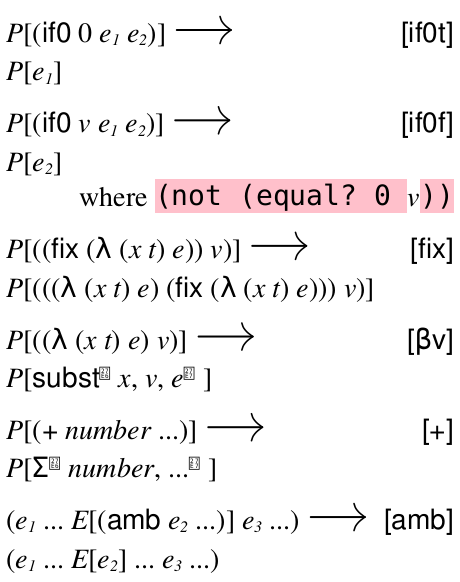
\includegraphics[scale=0.3]{fig/red-pink.png}
  \caption{The initial rendering of the \texttt{red} reduction relation}
  \label{fig:red-pink}
\end{figure}

To output the picture in a PostScript file, one can use the \texttt{pict}
Racket library, which allows for further customizations that we will skip:
{
  \small
\begin{verbatim}
(require pict)
(scale (vl-append
        20
        (language->pict Ev)
        (redeuction-relation-> pict red))
        3/2)
;; => outputs the image to a .ps in the current directory
\end{verbatim}
}

Note that we have a highlighted function that Redex did not recognize
properly, since it is a default Racket function. To eliminate this highlighting,
we must turn the Racket function into a Redex metafunction. Or we can just
use \texttt{different}, that is already a metafunction, defined earlier. Thus,
the snippet below can be either used to replace the \texttt{if0false} rule
in \texttt{red} or used and typeset per se:
{
  \small
\begin{verbatim}
(define if0-false-rule
  (reduction-relation Ev
    #:domain p
    (--> (in-hole P (if0 v e_1 e_2))
         (in-hole P e_2)
         (side-condition (term (different v 0)))
         "if0false")))

;; typeset it separately
(render-reduction-relation if0-false-rule)
\end{verbatim}
}
\noindent which gives figure \ref{fig:if0false}.

\begin{figure}[!htb]
  \centering
  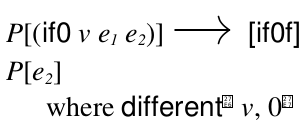
\includegraphics[scale=0.3]{fig/if0false.png}
  \caption{Fixed pink highlight for \texttt{if0false} rule}
  \label{fig:if0false}
\end{figure}

Further tweaks can be made, e.g.\ to use more or better Unicode symbols,
but we will skip them.

We close this section by mentioning \texttt{traces}, which is a great tool
embedded in Redex that shows all the reduction paths for a certain term,
according to the reduction relation specified. Its dependency is
\href{https://graphviz.org/}{Graphviz}, an open-source tool for interactive
graph visualization. Thus, the call:
{
  \small
\begin{verbatim}
(traces red
  (term ((+ (amb 1 2)
            (amb 10 20)))))
\end{verbatim}
}
\noindent shows all the reduction steps, with labels, to fully reduce the specified
term. In this case, we get figure \ref{fig:traces-amb}.

This figure was exported from Graphviz, which also provides some customization
tools, along with a \qq{Fully Reduce} button, which expands the figure until
the final result, which is \texttt{(11 12 21 22)}. This is shown in
figure \ref{fig:traces-amb-full} (notice the extra two bottom rows).
The tool also reports the various reduction paths displayed, in this case
(with the full reduction) the number being 26.

\newpage
\begin{landscape}
  \centering
  \begin{figure}[!h]
    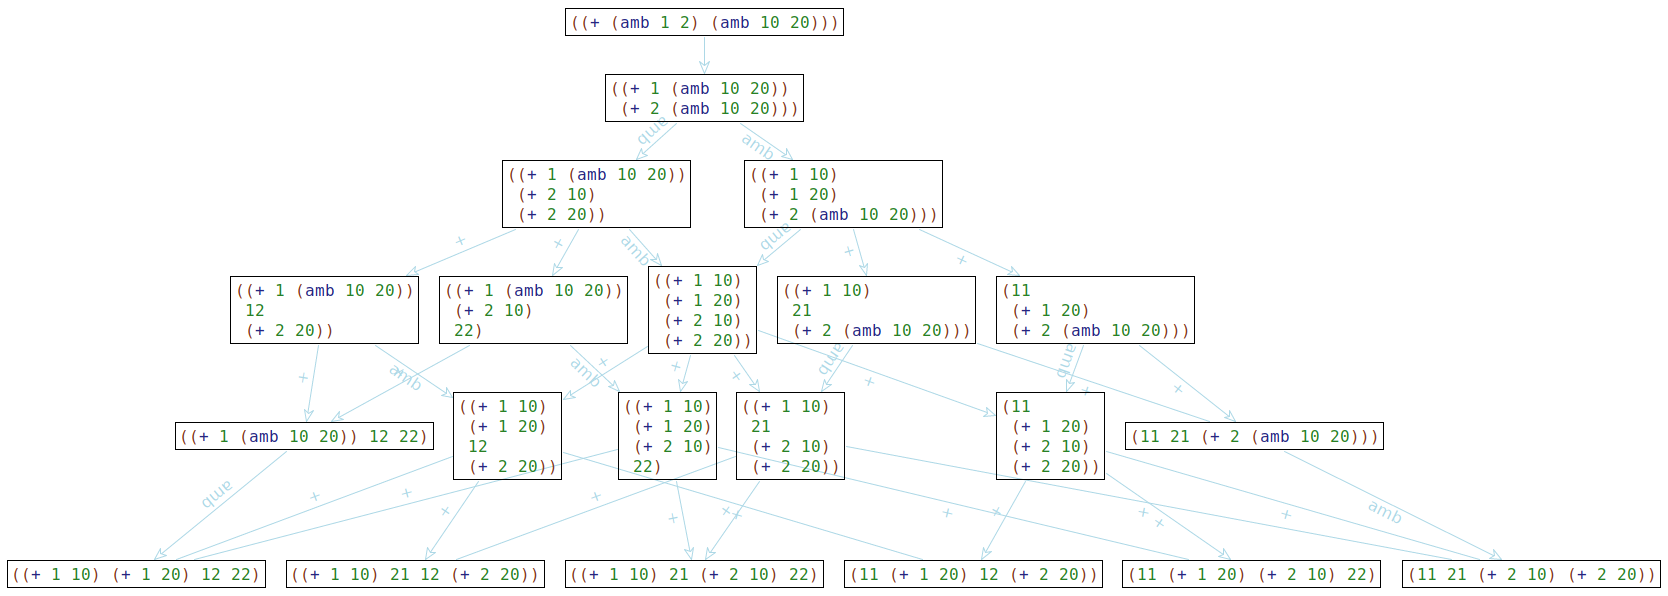
\includegraphics[scale=0.4]{fig/traces-amb.png}
    \caption{The incomplete reduction steps using \texttt{red} \\
      for \texttt{(term ((+ (amb 1 2) (amb 10 20))))}}
    \label{fig:traces-amb}
  \end{figure}
\end{landscape}

\newpage
\begin{landscape}
  \centering
  \begin{figure}[!h]
    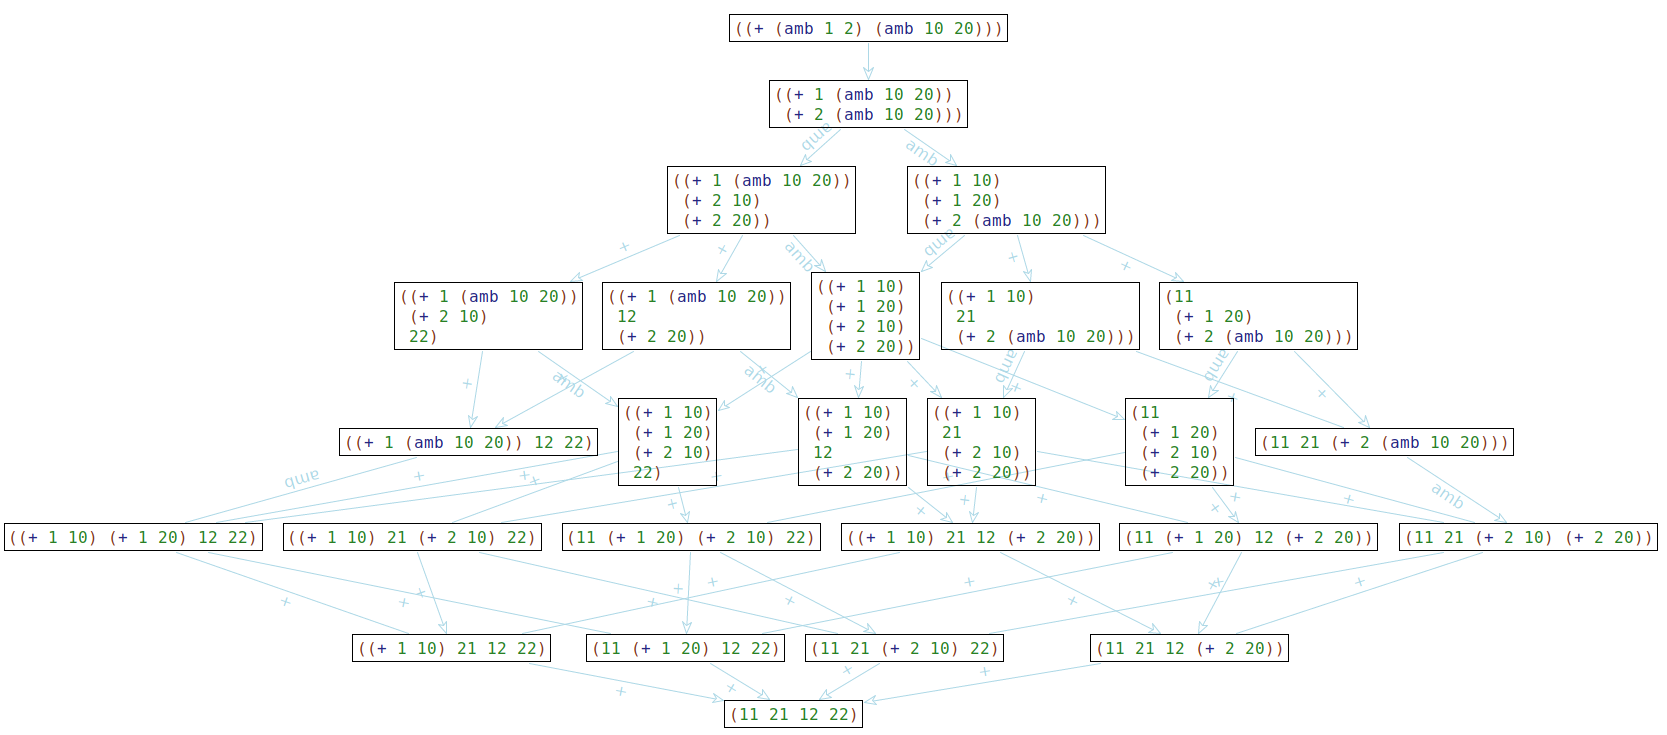
\includegraphics[scale=0.4]{fig/traces-amb-full.png}
    \caption{The full reduction steps using \texttt{red} \\
      for \texttt{(term ((+ (amb 1 2) (amb 10 20))))}}
    \label{fig:traces-amb-full}
  \end{figure}
\end{landscape}

%%%%%%%%%%%%%%%%%%%%%%%%%%%%%%%%%%%%%%%%%%%%%%%%%%%%%%%%%%%%%%%%%%%%%%

\section{The POPL case}

We now turn to the more \qq{serious} use of Redex, namely that presented at
POPL 2012 and detailed in \cite{popl} and \cite{sewpr}.

Having explained in detail the simple, but comprehensive example above,
we now jump straight into the action. As such, we first define the simple
language \texttt{Lambda-c}, encompassing basic (untyped) lambda calculus,
plus \texttt{call/cc}, then extend it with evaluation contexts (and holes),
plus the corresponding reduction relations.

So basically, we start with the following simple BNF grammar:
\begin{align*}
  e ::&= (e \ e \ \dots) \\
      &| \ x \\
      &| \ (\lambda (x \dots). e) \\
      &| \ \texttt{call/cc} \\
      &| \ + \\
      &| \ \texttt{number},
\end{align*}
which is readily written in Redex as:
{
  \small
\begin{verbatim}
#lang racket
(require redex)

(define-langauge Lambda-c
  (e (e e ...)
     x
     (lambda (x ...) e)
     call/cc
     +
     number)
  (x variable-not-otherwise-mentioned))
\end{verbatim}
}

Then we extend it with contexts, formally written in BNF as:
\begin{align*}
  e ::&= \dots | (A \ e) \\
  v ::&= (\lambda (x \dots). e) \\
      &| \ \texttt{call/cc} \\
      &| \ + \\
      &| \ \texttt{number} \\
  E ::&= (v \dots E \ e \dots) \\
      &| \ [ \ ]
\end{align*}
and then in Redex as:
{
  \small
\begin{verbatim}
(define-extended-language
  Lambda-c/red Lambda-c
    (e ... (A e))
    (v (lambda (x ...) e)
       call/cc
       +
       number)
    (E (v ... E e ...)
       hole))
\end{verbatim}
}
Aside from the \emph{evaluation context} \texttt{E}, we have now introduced the
\emph{abortion context} \texttt{A}, whose role can be seen in the reduction rules
which follow below, first presented in a mathematical form, then in Redex:
\begin{itemize}
\item $ E[(A e)] \to e $ (\emph{abort});
\item $ E[(\texttt{call/cc} v)] \to E[(v (\lambda x . (A E[x])))] $,
  for $ x $ a \emph{fresh variable} (\emph{call/cc});
\item $ E[((\lambda (x \dots_1).e)v \dots_1)] \to E[e \{ x := v, \dots \}] $
  (\emph{$\beta$-reduction});
\item $ E[(+ \texttt{number} \dots)] \to E[\Sigma (number \dots)] $ ($\Sigma$).
\end{itemize}
Note that the rule for $ \beta $-reduction used two kinds of ellipses, to show
that after applying the rule, the rest of the computation could be different.
Also, the \texttt{call/cc} reduction basically shows how the call with current
continuation is equivalent to some lambda expression, in which the special context
for {\color{red} \textbf{abortion}} was used.
\todo[inline,noline,backgroundcolor=green!40]{abort (exit) or continue??}

Now in Redex:
{
  \small
\begin{verbatim}
(define red
  (reduction-relation
   Lambda-c/red
   #:domain e
   (--> (in-hole E (A e))
        e
        "abort")
   (--> (in-hole E (call/cc v))
        (in-hole E (v (lambda (x) (A (in-hole E x)))))
        (fresh x)
        "call/cc")
   (--> (in-hole E ((lambda (x ..._1) e) v ..._1))
        (in-hole E (subst e (x v) ...))
        "beta-reduction")
   (--> (in-hole E (+ number ...))
        (in-hole E (Sigma number ...))
        "sum")))
\end{verbatim}
}

We assume that the metafunctions \texttt{Sigma} and \texttt{subst} are already
defined, as in the previous section.

One more extension we can add is to allow the reductions to happen anywhere
in redexes, since as defined in the extension \texttt{Lambda-c/red}, the first
item of an expression in an \texttt{E}-context is a value \texttt{v}:
{
  \small
\begin{verbatim}
(define-extended-language
  anywhere-Lambda-c Lambda-c/red
  (E (e ... E e ...)
     hole))

;; extend the reductions by copying them
(define anywhere-red
  (extend-reduction-relation
    red anywhere-Lambda-c))
\end{verbatim}
}

%%%%%%%%%%%%%%%%%%%%%%%%%%%%%%%%%%%%%%%%%%%%%%%%%%%%%%%%%%%%%%%%%%%%%%
\section{Extensive and Randomized Tests}

Randomized testing in Redex is detailed in \cite{randomplt}. Also, as it is
explained in \cite{popl}, Redex (and Racket) supports QuickCheck tests,
in the style of the well-known combinator library initially developed
in and for Haskell (\cite{quickcheck}).

Before going into more details, we mention a simple test that can be run,
using \texttt{redex-check}. The general syntax and more complex use is
explained at \cite{redex-check}. We will first use the form:
\[
  \texttt{(redex-check G n e)},
\]
in which the boolean-valued expression \texttt{e} is seen as a predicate
which is universally quantified over \texttt{n} and evaluates it for
random terms that are generated from the non-terminal \texttt{n} belonging
to the grammar \texttt{G}. Tweaks can be added, such as seeds for the
random generation, trace printing, number of attempts, restrictions for the
generated terms etc., but we will explore them later. First, a quick example:
{
  \small
\begin{verbatim}
(redex-check
  Lambda-c/red e
    (or (redex-match Lambda-c/red v (term e))   ; is it a term OR
        (cons?                                  ; is it a list
            (apply-reduction-relation red       ; after reducing ?
                (term e)))))
;; => counterexample found after 9 attempts: S
\end{verbatim}
}

The example checks whether in the grammar \texttt{G} of the language
\texttt{Lambda-c/red}, when quantifying over expressions \texttt{e},
what follows can be an expression \texttt{e}. Then, the disjunction
(which must be a boolean-valued function) checks whether either
\texttt{term e} is a value \texttt{v} in the language or after
reducing it using \texttt{red} it is still a list.

The check reports that a free variable is a counterexample for the test,
of course, since it's neither reducible, nor a value. This can be fixed
by adding a special reduction relation to spot precisely free variables:
{
  \small
\begin{verbatim}
;; ... add to red ...
(--> (in-hole E x)
     error
     "free variable")
;; ...
\end{verbatim}
}


%%% Local Variables:
%%% mode: latex
%%% TeX-master: "../redex"
%%% End:
